\documentclass{ximera}

\begin{document}

\begin{question}
  Find 
  \[
  \displaystyle \lim_{x\to 2} f(x)
  \]
  where
  \[
  f(x) = \left\{\begin{array}{cl} x+2 & x\leq 2, \\ 3x-5 & x>2. \end{array}\right.
  \]
  \begin{solution}
    \begin{hint}
     Both $x+2$, for $x\le2$, and $3x-5$, for $x>2$ are continuous on their respective domains. However, for the limit $\lim\limits_{x\to2}f(x)$ to exist, both the left-hand and the right-hand limits must exist and be equal.
    \end{hint}
     \begin{hint}
    	Take a look at the graph of the function
    \begin{center}
     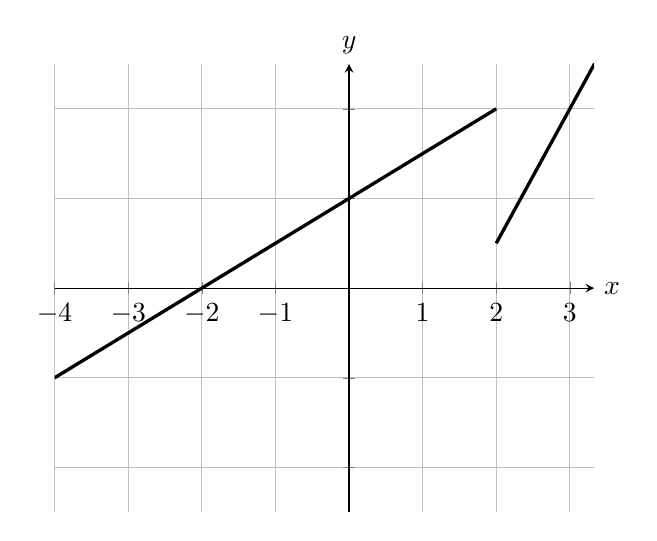
\begin{tikzpicture}
	\begin{axis}
	[ymin=-5,ymax=5, axis lines=center,xlabel=$x$,ylabel=$y$,every axis y 
	label/.style={at=(current axis.above origin),anchor=south},every axis x label/.style={at=(current axis.right of origin),anchor=west},
	domain=-4:4,
	yticklabels={},
	ymajorgrids=true,
	grid = major
	]
	\addplot[domain=-4:2,very thick,smooth,samples=300]
	{2+\x};
	\addplot[domain=2:4,very thick,smooth,samples=300]
	{3*\x-5};
	\end{axis}
       \end{tikzpicture}      
      \end{center} 
    \end{hint}
    \begin{hint}
     Evaluating $\lim\limits_{x\to2^{+}}f(x)$ we see that it tends to $6-5=1$. This follows because, for $x>2$, we are on the piece of $f(x)$ given by $3x-5$ and the limit $\lim\limits_{x\to2}3x-5=1$, certainly. On the other hand, evaluating $\lim\limits_{x\to2^{-}}f(x)$ we see it tends to $2+2=4$. This follows because, for $x\le2$, we are on the piece of $f(x)$ given by $x+2$ and the limit $\lim\limits_{x\to2}x+2=4$, certainly. These are not equal.
    \end{hint} 
    \answer{\text{Limit does not exist}}.
  \end{solution}
\end{question}

\end{document}